\chapter{System Design}
\label{ch:design}

\section{Design of the Reproduction Pipeline}
The reproduction is a file-based pipeline in which every stage reads and writes files, so any stage can be re-run alone (Figure~\ref{fig:pipeline}). BigQuery extraction aggregates the public Ethereum tables on the server so that only compact tables are downloaded. A DuckDB build turns those tables into a top-200 neighbour graph. A core-set selection and node2vec training stage produces embeddings, which propagation or the dynamic variant extend to all addresses. A random forest combines embeddings with behavioural features and public labels, and an evaluation stage regenerates the paper's tables and figures.

\begin{figure}[H]
\centering
\resizebox{\textwidth}{!}{%
\begin{tikzpicture}[box/.style={draw,rounded corners,align=center,minimum height=9mm,minimum width=3.1cm,font=\footnotesize,fill=blue!6},
  arr/.style={-{Stealth[length=2mm]},thick}]
\node[box] (bq) at (0,0) {BigQuery extraction\\(public Ethereum tables)};
\node[box] (gr) at (3.9,0) {Graph build\\(DuckDB, top-200)};
\node[box] (co) at (7.8,0) {Core set /\\universe selection};
\node[box] (tr) at (11.7,0) {node2vec training\\(streaming walks)};
\node[box,fill=green!8] (em) at (11.7,-1.9) {Embeddings:\\propagation or dynamic};
\node[box] (rf) at (7.8,-1.9) {Random forest\\risk model};
\node[box] (ev) at (3.9,-1.9) {Evaluation\\(Tables II--IV, figures)};
\node[box] (fe) at (7.8,-3.8) {Behavioural\\features (66 cols)};
\node[box] (lb) at (11.7,-3.8) {Public labels\\(audited)};
\draw[arr] (bq)--(gr); \draw[arr] (gr)--(co); \draw[arr] (co)--(tr); \draw[arr] (tr)--(em);
\draw[arr] (em)--(rf); \draw[arr] (rf)--(ev); \draw[arr] (fe)--(rf); \draw[arr] (lb)--(rf);
\draw[arr] (bq) |- ([yshift=-1mm]fe.west);
\end{tikzpicture}}
\caption{Overview of the reproduction pipeline. Every stage reads and writes files.}
\label{fig:pipeline}
\end{figure}

\section{Architecture of CryptoTrace}
CryptoTrace is organised as a pipeline of modules with plain data interfaces: a complaint enters on the left, and a case file and dashboard leave on the right. A label store feeds the attribution step, and a benchmark harness sits beside the pipeline. Figure~\ref{fig:arch} shows the modules; solid boxes are built and exercised, dashed boxes are designed but pending. The same structure is drawn by the application's System page from a data file (\code{architecture.py}), so the interface can never show a module that does not exist.

\begin{figure}[H]
\centering
\resizebox{\textwidth}{!}{%
\begin{tikzpicture}[
  m/.style={draw,rounded corners,align=center,minimum height=9mm,minimum width=3.0cm,font=\footnotesize,fill=blue!6},
  p/.style={draw,dashed,rounded corners,align=center,minimum height=9mm,minimum width=3.0cm,font=\footnotesize,fill=gray!8},
  pa/.style={draw,rounded corners,align=center,minimum height=9mm,minimum width=3.0cm,font=\footnotesize,fill=yellow!14},
  hd/.style={font=\footnotesize\bfseries},
  arr/.style={-{Stealth[length=2mm]},thick}]
\node[hd] at (0,3.7) {INTAKE}; \node[hd] at (4,3.7) {DATA LAYER}; \node[hd] at (8,3.7) {ENGINES}; \node[hd] at (12,3.7) {OUTPUT}; \node[hd] at (16,3.7) {EVALUATION};
\node[pa] (intake) at (0,2.4) {Complaint intake\\(partial)};
\node[pa] (adapter) at (4,2.4) {Chain adapter\\(partial)};
\node[m]  (cache)   at (4,1.0) {Edge cache\\(SQLite)};
\node[m]  (labels)  at (4,-0.4) {Label store\\(with provenance)};
\node[m]  (tracing) at (8,2.4) {Tracing engine\\TTR-lite, Haircut, BFS};
\node[m]  (attr)    at (8,1.0) {Attribution engine\\(terminals, sweep rule)};
\node[m]  (typ)     at (8,-0.4) {Typology engine\\(pattern tags)};
\node[p]  (risk)    at (8,-1.8) {Risk model\\(RiskSEA, pending)};
\node[p]  (dex)     at (8,-3.2) {DEX pass-through,\\cross-chain (pending)};
\node[m]  (case)    at (12,2.4) {Case file\\(JSON per trace)};
\node[pa] (report)  at (12,1.0) {Investigator\\report (partial)};
\node[m]  (dash)    at (12,-0.4) {Dashboard \& API\\(FastAPI + React)};
\node[p]  (alerts)  at (12,-1.8) {Alerts / watchlist\\(pending)};
\node[m]  (bench)   at (16,2.4) {Benchmark\\documented cases};
\draw[arr] (intake)--(adapter); \draw[arr] (adapter)--(cache); \draw[arr] (cache.east)--(tracing.south west);
\draw[arr] (labels.east)--(attr.south west); \draw[arr] (tracing)--(attr); \draw[arr] (attr)--(typ);
\draw[arr] (typ.east)--(case.south west); \draw[arr] (attr.east)--(case.west); \draw[arr] (case)--(report); \draw[arr] (case.south)--(dash.north);
\draw[arr] (case.east)--(bench.west);
\draw[arr,dashed] (risk.east)--(case.south west); \draw[arr,dashed] (dex.north)--(tracing.south);
\draw[arr,dashed] (dash)--(alerts);
\end{tikzpicture}}
\caption{CryptoTrace architecture. Solid: built and exercised by the benchmark cases; yellow: partly built; dashed: designed but pending.}
\label{fig:arch}
\end{figure}

\begin{table}[H]
\centering\small\singlespacing
\begin{tabular}{p{3.2cm} p{2.1cm} p{7.6cm}}
\toprule
\textbf{Module} & \textbf{Status} & \textbf{Role and limit}\\
\midrule
Complaint intake & partial & Takes a wallet, window and strategy through the API; batch import and SAHYOG/NCRP integration are pending.\\
Chain adapter & partial & Ethereum external ETH transfers via BigQuery; internal transfers, ERC-20 and other chains pending.\\
Edge cache & live & SQLite store of every fetched neighbourhood; re-runs cost nothing.\\
Label store & live & 372 exchange, 5\,594 known-bad, 123 sanctioned, 4 mixer pools and 1 DEX (curated) addresses, each with provenance.\\
Tracing engine & live & TTR-lite plus the Haircut and BFS baselines.\\
Attribution engine & live & Labeled stops, deposit-sweep rule, unlabeled hub guard.\\
Typology engine & live & Zero-out, fan-out, fan-in, peel and fast-hop tags.\\
Risk model & planned & RiskSEA reproduction exists offline; not wired in.\\
DEX pass-through & planned & Needs the BigQuery traces table (internal transfers).\\
Cross-chain & planned & Needs bridge-event matching.\\
Case file & live & One JSON per trace with nodes, edges, destinations, paths, tags, warnings, events.\\
Investigator report & partial & Printable view live; standard-format export pending.\\
Dashboard \& API & live & FastAPI with live event streaming; React application.\\
Alerts / watchlist & planned & Needs a live feed.\\
Benchmark & live & Compares strategies on documented cases.\\
\bottomrule
\end{tabular}
\caption{The fifteen modules of CryptoTrace and their status.}
\label{tab:modules}
\end{table}

\section{Data Model}
Everything the engines do is expressed in terms of one structure, the \emph{Edge}: a single on-chain transfer, directed, timed and valued. A different chain only needs a different provider that yields Edges.

\begin{table}[H]
\centering\small\singlespacing
\begin{tabular}{p{2.6cm} p{4.0cm} p{6.4cm}}
\toprule
\textbf{Structure} & \textbf{Fields} & \textbf{Meaning}\\
\midrule
Edge & src, dst, eth, ts, blk, tx & One transfer: sender, receiver, value in ETH, Unix time, block number, transaction hash.\\
Label & kind, name, source & What an address is (exchange, mixer, sanctioned, bad, dex) and where that knowledge came from.\\
FetchResult & edges, degree, queries, bytes\_billed, cache\_hits & What one provider call returns: transfers, the true in/out degree before the per-node cap, and cost counters.\\
TraceParams & alpha, beta, epsilon, max\_rounds, min\_eth, hub\_degree, time\_respecting, top\_k, bfs\_depth, max\_frontier & The algorithm's parameters (defaults 0.15, 0.8, $10^{-3}$, 8, 0.01 ETH, 3000, true, 200, 2, 300).\\
TraceEvent & round, kind, nodes, edges, info & One animation frame: start, expand, absorb or done, with the round's frontier, residual and cost counters.\\
\bottomrule
\end{tabular}
\caption{Core data structures.}
\label{tab:datamodel}
\end{table}

The result of a trace (the \emph{case file}) contains: the nodes with their role (source, intermediate, terminal, upstream), label, depth, rank, share and pattern tags; the edges with role (forward or backward) and share; the terminals with type, share, estimated ETH, depth, first-arrival time, confidence and evidence path; the statistics (rounds, queries, bytes billed, cache hits, seconds); the warnings; and the full event log used by the interface to replay the search.

\section{Data Layer Design}
\subsection{One query per hop}
Tracing asks for the neighbourhood of a few addresses at a time. Each search round is therefore one BigQuery query against the public \code{transactions} table, returning at most the 200 largest transfers per address and direction. This keeps the cost independent of how large the chain is. The query (Listing~\ref{lst:hopsql}) filters by a time window so BigQuery can prune partitions, drops dust below \code{min\_eth}, and uses a window function to keep the top-$k$ per node and direction while also returning the true degree, which the attribution engine uses to recognise busy hubs.

\begin{figure}[H]
\centering\footnotesize
\begin{minipage}{0.97\textwidth}
\begin{verbatim}
WITH e AS (          -- transfers touching the requested nodes
  SELECT hash AS tx, from_address AS src, to_address AS dst,
         CAST(value AS FLOAT64)/1e18 AS eth,
         UNIX_SECONDS(block_timestamp) AS ts, block_number AS blk
  FROM `bigquery-public-data.crypto_ethereum.transactions`
  WHERE block_timestamp >= TIMESTAMP_SECONDS(@t0)   -- prunes partitions
    AND block_timestamp <  TIMESTAMP_SECONDS(@t1)
    AND to_address IS NOT NULL AND value > 0
    AND (from_address IN UNNEST(@nodes)
         OR to_address IN UNNEST(@nodes))
), ends AS (         -- one row per (node, direction)
  SELECT src AS node,'out' AS dir,tx,src,dst,eth,ts,blk
    FROM e WHERE src IN UNNEST(@nodes)
  UNION ALL
  SELECT dst AS node,'in' AS dir,tx,src,dst,eth,ts,blk
    FROM e WHERE dst IN UNNEST(@nodes)
)
SELECT node,dir,tx,src,dst,eth,ts,blk,
       COUNT(*) OVER (PARTITION BY node,dir) AS deg  -- true degree
FROM ends WHERE eth >= @min_eth
QUALIFY ROW_NUMBER() OVER (PARTITION BY node,dir
                           ORDER BY eth DESC) <= @k   -- top-k
\end{verbatim}
\end{minipage}
\caption{The per-hop query (abridged from the implementation).}
\label{lst:hopsql}
\end{figure}

\subsection{Cache, cost control and the provider interface}
The provider is the only component that talks to BigQuery. It stores every fetched neighbourhood in a SQLite database keyed by the minimum value, the per-node cap and the end of the window; an address is therefore fetched at most once per configuration, and a later request for an earlier start time triggers a re-fetch of only that address. Four controls bound the spend: (i)~a dry run reports the bytes a query would scan before anything is billed; (ii)~every job carries a \code{maximum\_bytes\_billed} cap of 40\,GiB; (iii)~the provider refuses to start a query that would take the total for one trace over a 30\,GiB budget; and (iv)~in \emph{cache-only} mode a request for an address that was never fetched raises a clear error instead of silently spending. The engines always request edges from the start of the incident window and decide themselves which are time-consistent, so the provider never filters by time and the time-respecting switch is real. A second provider holds a fixed edge list in memory for tests and replays.

\subsection{Label store}
The label store maps an address to a \emph{kind} and a \emph{name} and records the source of every label. It is loaded from public files: Etherscan-derived exchange and phishing/hack lists, the OFAC sanctions list, and a small curated list. The curated list holds the four Tornado Cash pool addresses (each verified on-chain to receive a single fixed denomination of 0.1, 1, 10 or 100 ETH), the EtherDelta contract (curated from public knowledge and marked \emph{unverified on-chain}) and the Yobit.net wallet printed in the textbook's case study. Figure~\ref{fig:label_store} shows the counts.

\begin{figure}[H]
\centering
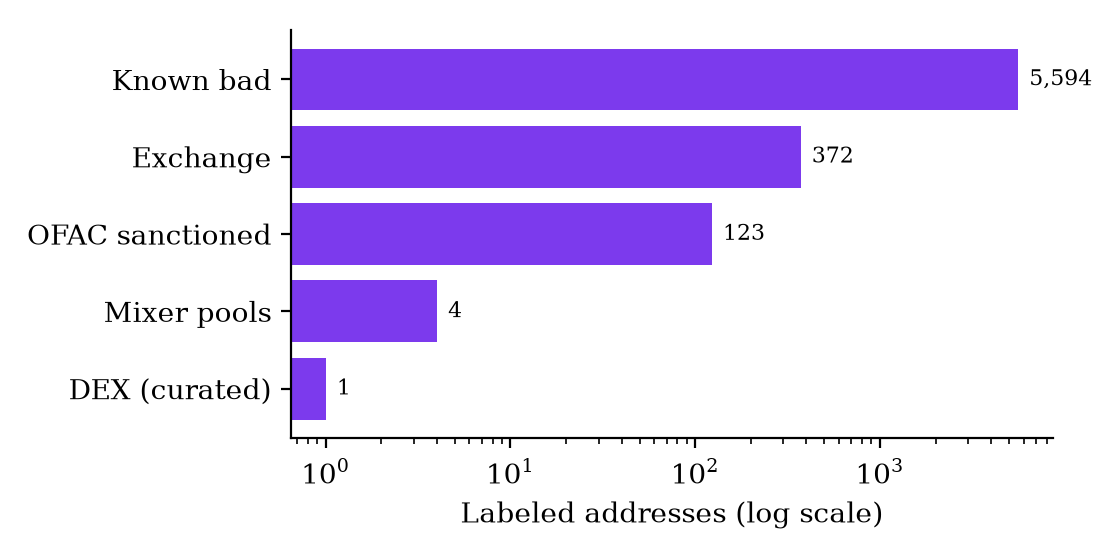
\includegraphics[width=0.78\textwidth]{figs/label_store.png}
\caption{Labeled addresses by kind in the label store (log scale).}
\label{fig:label_store}
\end{figure}

\section{Tracing Engine Design}
\subsection{Idea}
The tracer treats the reported wallet as holding 100\% of an unexplained quantity, the \emph{residual}, and repeatedly pushes residual along transfers to the next accounts, in proportion to value, until the residual left unexplained is negligible or the funds reach a service. Two quantities travel together. The \emph{rank} measures relevance to the source, decays with distance and decides which accounts are expanded next. The \emph{share} estimates the fraction of the source's funds that reached an account and is what the report states.

\subsection{TTR-lite formulation}
Let $r(v)$ be the residual at account $v$, initialised to $r(s)=1$ at the source $s$, and let $\alpha,\beta,\epsilon$ be the parameters of Table~\ref{tab:datamodel}. In each round every account with $r(v)>\epsilon$ that is not a terminal or an upstream account is expanded, highest residual first, at most 300 per round. For an expanded account $v$ that first received funds at time $a(v)$:
\begin{align}
F(v)&=\{(v\to u,x,t):t\ge a(v)\}, & B(v)&=\{(w\to v,x,t):t<a(v)\},\\
\mathrm{rank}(v) &\mathrel{+}= \alpha\, r(v),\\
r(u) &\mathrel{+}= (1-\alpha)\,\beta\, r(v)\,\frac{x}{\sum_{F(v)}x} && \forall\,(v\to u,x,t)\in F(v),\\
r(w) &\mathrel{+}= (1-\alpha)(1-\beta)\, r(v)\,\frac{x}{\sum_{B(v)}x} && \forall\,(w\to v,x,t)\in B(v).
\end{align}
The four ideas taken from the literature are visible here. \emph{Tracing tendency}: $\beta$ of the residual goes forward along outflows and $1-\beta$ backward along inflows. \emph{Weighted pollution}: the split is proportional to the amount transferred. \emph{Temporal reasoning}: forward transfers must occur at or after the funds arrived, and backward transfers strictly before, so the transfer on which the funds arrived is never walked backwards. \emph{Token redirection} through swaps is not implemented in the prototype because it handles ETH only. In parallel, a pending share $\sigma(v)$ is split by the same forward fractions, $\sigma(u)\mathrel{+}=\sigma(v)\,x/\sum_{F(v)}x$, and is the quantity reported as ``share of funds''. If an account has no forward or no backward transfers, all of its residual goes the other way.

\subsection{Baselines}
\textbf{Haircut taint} carries a sender's tainted share forward in proportion to value and stops when the remaining taint is below a threshold; it is forward-only, has no ranking and no backward pass. \textbf{Blind BFS} follows every outflow of every discovered account to a fixed depth (two, as in the literature), ignoring time and amount; shares are split uniformly and exist only so the comparison table can be filled. Both baselines use the same provider, terminals and result builder as TTR-lite, so differences in the comparison come from the search strategy alone.

\section{Attribution Design}
\subsection{Terminals}
A \emph{terminal} is an account where tracing stops because the funds reached a service. Labeled exchanges, mixers, sanctioned addresses and DEX contracts stop the trace immediately, without fetching their (huge) neighbourhood. Two further terminals are inferred.

\paragraph{Exchange deposit address (sweep rule).} Public lists tag an exchange's hot wallets but rarely its customer deposit addresses, which an exchange creates by the thousand and \emph{sweeps} into its hot wallet. An unlabeled account $v$ is classified as a deposit address of exchange $X$ if, among its outflows within 48 hours of the funds arriving, at least 80\% of the value goes to labeled wallets of $X$ and the outflows go to at most three recipients. The result carries \emph{medium} confidence and the label ``inferred''. Figure~\ref{fig:sweep} shows the pattern.

\begin{figure}[H]
\centering
\resizebox{0.9\textwidth}{!}{%
\begin{tikzpicture}[n/.style={draw,circle,minimum size=9mm,font=\footnotesize,align=center},
  arr/.style={-{Stealth[length=2mm]},thick}, lab/.style={font=\scriptsize,midway,above}]
\node[n,fill=cyan!20] (s) at (0,0) {source};
\node[n,fill=blue!10] (a) at (3,0) {hub};
\node[n,fill=teal!20] (d1) at (6.3,1.5) {dep$_1$};
\node[n,fill=teal!20] (d2) at (6.3,0) {dep$_2$};
\node[n,fill=teal!20] (d3) at (6.3,-1.5) {dep$_n$};
\node[n,fill=green!25,minimum size=13mm] (x) at (9.8,0) {\scriptsize exchange\\\scriptsize hot wallet};
\draw[arr] (s)--(a) node[lab] {2\,298 ETH};
\draw[arr] (a)--(d1) node[lab,sloped] {100 ETH};
\draw[arr] (a)--(d2) node[lab] {100 ETH};
\draw[arr] (a)--(d3) node[lab,sloped,below] {100 ETH};
\draw[arr] (d1)--(x); \draw[arr] (d2)--(x); \draw[arr] (d3)--(x);
\node[font=\scriptsize,align=center] at (8.0,-2.6) {each deposit address forwards $\ge 80\%$ of its\\outflow to the exchange within 48 hours};
\end{tikzpicture}}
\caption{The deposit sweep pattern that the attribution engine looks for.}
\label{fig:sweep}
\end{figure}

\paragraph{Unlabeled service hub.} An unlabeled account with more than 3\,000 transfers in the window is treated as a service (a pool, a payment processor or an exchange wallet that no list names). The trace stops there with \emph{low} confidence and the account is flagged for manual review, because following funds through such an account is guesswork.

\subsection{Confidence}
Labeled exchanges, mixers and sanctioned addresses carry high confidence, since the label itself is public knowledge. A DEX contract and an inferred exchange deposit address carry medium confidence (the label is curated, or the link is inferred). An unlabeled hub carries low confidence.

\subsection{Evidence paths}
For each terminal the engine reports the time-ordered chain of real transactions from the source that carries the largest share. Starting from the source, it scans all forward edges in time order and keeps, for each account, the best score so far, where the score of an edge is the score of its sender times the fraction of the sender's outflow that the edge carries; an edge is usable only if it occurs after the funds reached its sender. Walking the predecessor links back from the terminal gives the path. This is a dynamic program over the time-sorted edge list.

\section{Typology Design}
The typology engine tags accounts of the traced subgraph with simple rules that need no training data and can be read by an investigator.
\begin{itemize}
\item \textbf{Zero-out:} forwards at least 90\% of what it received within 24 hours (a pass-through bridge account).
\item \textbf{Fan-out:} sends to five or more different recipients within 24 hours (splitting or layering).
\item \textbf{Fan-in:} receives from five or more different senders (aggregation).
\item \textbf{Peel:} passes at least 70\% of the funds in one transfer and keeps or spreads a small remainder, repeatedly.
\item \textbf{Fast hop:} first outflow within one hour of the funds arriving.
\end{itemize}

\section{API Design}
The backend exposes a small REST interface and one streaming endpoint (Table~\ref{tab:api}). A trace runs as a background job: the client posts the request, receives a job identifier, and opens a server-sent event stream that delivers one message per search round as it happens, followed by the final result or an error. Requests are validated: the engine must exist, an address must be a 40-hex-digit string, the dates must be in order and the window at most 120 days. In the default cache-only mode a request that needs data that was never fetched ends with a \code{cache\_miss} error that says so; live BigQuery access is available only if the server was started with a project identifier and credentials.

\begin{table}[H]
\centering\small\singlespacing
\begin{tabular}{p{1.3cm} p{5.6cm} p{6.0cm}}
\toprule
\textbf{Method} & \textbf{Path} & \textbf{Purpose}\\
\midrule
GET & \code{/api/health} & Liveness, label counts, whether live mode is available.\\
GET & \code{/api/meta} & Engines, default parameters, label counts, data limits.\\
GET & \code{/api/cases} & Benchmark cases with headline findings, available engines and first-fetch cost.\\
GET & \code{/api/cases/\{id\}/trace/\{engine\}} & Stored case file for a case and strategy.\\
GET & \code{/api/cases/\{id\}/compare} & Strategy comparison rows for a case.\\
POST & \code{/api/trace} & Start a trace (case or custom wallet); returns a job identifier.\\
GET & \code{/api/jobs/\{id\}/stream} & Server-sent events: round events, then the result or error.\\
GET & \code{/api/architecture} & Modules, flows and animation stages drawn by the System page.\\
\bottomrule
\end{tabular}
\caption{REST and streaming endpoints.}
\label{tab:api}
\end{table}

\section{User Interface Design}
\label{sec:design-group}
The interface is a single-page React application with six pages reached from a left rail: \emph{Overview}, \emph{System}, \emph{Trace Lab}, \emph{Compare}, \emph{Gaps} and \emph{Report}. The design follows four rules.
\begin{enumerate}
\item \textbf{Show the mechanism, not only the answer.} The Trace Lab animates the search round by round on a force-directed canvas, with a counter of the share of funds still unexplained, so the audience sees the algorithm at work.
\item \textbf{One finding per receiving entity.} Twenty-nine deposit addresses that feed one exchange are one finding with an expandable list, not twenty-nine cards.
\item \textbf{Colour carries meaning.} Source, intermediate, exchange or deposit, mixer, DEX and unlabeled service each have one colour, repeated in the legend.
\item \textbf{State the limits where the result is shown.} Inferred links, curated labels and the data limits appear next to the findings and in the report.
\end{enumerate}
The Trace Lab has three columns: a control column (demo guide, case picker, strategy, parameters), the animated graph with a playback bar, and a result column with three tabs (Findings, Inside the engine, Account). It supports keyboard shortcuts for presenting (Space, arrow keys, F, R) and collapses to narrower layouts at projector and tablet sizes. The animation is driven by the event log, so a stored case and a freshly streamed job behave identically.
